This section, freely inspired by the work of Bonneau, Faraut and Valent~\cite{Bonneau_2001}, is aimed at introducing the concept of self-adjoint extensions of an Hamiltonian operator. 
However, the choice of the free particle on the half-line is not arbitrary, as it represents our original problem where $a = 0$ is imposed. Consequently, we can verify the results obtained from the particle in the potential by considering the scenario where we force $a$ to vanish.

\paragraph*{Note:}
Since this problem is a specific case of a larger one, we know that it inherits its properties, including the important feature of scale invariance, which prohibits the existence of a ground state.\footnote{If we consider some particular boundary conditions, or we don't consider them at all.}

\vspace{4mm}
\noindent
Let's apply the previous analysis to the Hamiltonian operator \(H = -(\hbar^2/2m)d^2/dx^2\).
In this section, we initially approach the problem from a mathematical perspective, leading us to the discovery that there are infinitely many self-adjoint extensions parameterized by \(U(1\)), which corresponds to a phase. Only in the end will be demonstrated that, in this problem, the seemingly straightforward boundary conditions that we might choose intuitively as physicists make already $H$ self-adjoint, differently from what will happen in Section~\ref{section:xsqared_halfaxis}.

\clearpage

\subsection{The Self-adjoint Extensions}
In this section, we apply the previous theorem.

\subsubsection*{The Deficiency Indices}

Let us consider the Hilbert space $\mathcal{H} = \mathcal{L}^2(0,\infty)$
, and to use von Neumann's theorem, we have to determine the functions $\phi_{\pm}(x)$ given by:
\begin{equation} \label{eq:free_H}
    H^\dagger \phi_{\pm}(x) = - \frac{\hbar^2}{2m} \frac{d^2}{dx^2} \phi_{\pm}(x) = \pm \frac{\hbar^2}{2m} ik^2_0 \phi_{\pm}(x), \quad k_0 > 0
\end{equation}

\noindent
An easy integration gives:
\begin{equation*}
    \phi_{\pm} = a_{\pm}e^{k_{\pm}x} + b_{\pm}e^{-k_{\pm}x}, \quad k_{\pm} = \frac{1 \mp i}{\sqrt{2}} k_0 = e^{\mp i \pi/4} k_0
\end{equation*}

\noindent
Then we have to discuss what happens on our interval $[0,\infty)$, the positive semi-axis.
\paragraph{Note:}
For dimensional reasons, we have introduced the constant $k_0$, and, as we preannounced in Section~\ref{section:self_adjoint}, its introduction is compelled by the method.

\vspace{4mm}
\noindent
In the Hilbert space \(\mathcal{H} = \mathcal{L}^2(0, +\infty)\), we have normalized solutions to Eq.~\eqref{eq:free_H} given by:
\begin{align} \label{eq:freepart_eigenfun}
    \phi_{\pm} = b_{\pm}e^{-e^{\mp i \pi/4} k_0 x}, \quad b_\pm = e^{\mp i \pi /4} k_0 (= k_\pm)
\end{align}

\noindent
Since the $a_\pm$ terms grow exponentially, they're not integrable. This leads to deficiency indices \((1, 1)\), resulting in infinitely many self-adjoint extensions parametrized by \(U(1)\), such that $U = e^{i\theta}$ with $\theta \in [0,2\pi]$.
 
\clearpage

\subsubsection*{The Boundary Conditions}

To find the space that makes $H$ self-adjoint, we need to find the $\psi$ that satisfies Eq.~\eqref{eq:boundary_condition}. Defining $\Phi_\theta = \phi_+ + e^{i\theta} \phi_-$, we need the following to vanish:

\begin{align*}
    \langle \Phi_\theta | H \psi \rangle - \langle H \Phi_\theta |  \psi \rangle
     & = \frac{\hbar^2}{2m} \left(\langle \Phi_\theta | - \frac{d^2}{dx^2} \psi \rangle - \langle - \frac{d^2}{dx^2} \Phi_\theta |  \psi \rangle \right)                                                                 \\
     & =  \frac{\hbar^2}{2m} \left(\int_0^\infty -\overline{\Phi_\theta} \psi'' + \int_0^\infty \overline{\Phi_\theta''} \psi \right)                                                                      \\
     & = \frac{\hbar^2}{2m} \left((-\overline{\Phi_\theta} \psi')\Big|_0 + \int_0^\infty \overline{\Phi_\theta'} \psi' + \int_0^\infty \overline{\Phi_\theta''} \psi  \right)                              \\
     & = \frac{\hbar^2}{2m} \left((-\overline{\Phi_\theta} \psi' + \overline{\Phi_\theta'} \psi)\Big|_0 - \int_0^\infty \overline{\Phi_\theta''} \psi + \int_0^\infty \overline{\Phi_\theta''} \psi\right) \\
     & = \frac{\hbar^2}{2m} \left((-\overline{\Phi_\theta} \psi' + \overline{\Phi_\theta'} \psi)\Big|_0\right)
\end{align*}

\noindent
So we need: $\overline{\Phi_\theta}(0) \psi'(0) = \overline{\Phi_\theta'}(0) \psi(0)$ as $x \rightarrow 0$.

If we replace the values of $\Phi_\theta (0)$ and its derivative:
\begin{align*}
    \overline{\phi_+(0) + e^{i\theta} \phi_-(0)} \psi'(0) = \overline{\phi_+'(0) + e^{i\theta} \phi_-'(0)} \psi(0)
\end{align*}

\noindent
Computing the values of $\phi_\pm'$:
\begin{align*}
    \phi_\pm' (x) = -k_\pm b_\pm e^{-k_\pm x} = -k_\pm^2 e^{-k_\pm x}
\end{align*}

\noindent
So, evaluating everything at zero and substituting, the condition becomes:
\begin{align*}
    (\overline{k_+ + e^{i\theta}k_-}) \psi'(0) & = (\overline{-k_+^2 - e^{i\theta} k_-^2} )\psi(0) \\
    (k_- + e^{-i\theta}k_+) \psi'(0)           & = -(k_-^2 + e^{-i\theta} k_+^2 )\psi(0)
\end{align*}
Rearranging the terms
\begin{align*}
    \frac{\psi'(0)}{\psi(0)}
     & = - \frac{k_-^2 + e^{-i\theta} k_+^2}{k_- + e^{-i\theta}k_+}                                                                         \\
     & = - k_0 \frac{e^{i \pi /2} + e^{-i\theta} e^{- i \pi /2}}{e^{i \pi /4} + e^{-i\theta}e^{- i \pi /4}}                                 \\
     & = - k_0 \frac{e^{-i\theta/2}e^{i \pi /2} + e^{-i\theta/2} e^{- i \pi /2}}{e^{-i\theta/2}e^{i \pi /4} + e^{-i\theta/2}e^{- i \pi /4}} \\
     & = - k_0 \frac{\cos(\theta/2 + \pi/2)}{\cos(\theta/2 + \pi/4)}
\end{align*}

\noindent
The term on the right of this equation can assume every real value for $\theta \in [0,2\pi]$.

\clearpage
\noindent
So the final form of the boundary conditions is:

\begin{equation} \label{half_BC}
    \psi(0) = x_0 \psi'(0)  \quad x_0 \in \mathbb{R}
\end{equation}

\noindent
The boundary condition \(\psi'(0) = 0\) corresponds to \({x_0} = \infty\). The most commonly used extension in physics is \({x_0} = 0\), which implies \(\psi(0) = 0\). The latter derives from the infinite potential for $x<0$ and the continuity of the wave function.

\paragraph{Note:}
The ${x_0}$ that characterizes the boundary condition of its corresponding self-adjoint extension is not dimensionless; in fact, it has the dimension of length. Therefore, we have introduced a new parameter, and the dimensional problem of constructing a formula for the eigenvalues is solved. We can say that now that we've our problem provided with boundary conditions that make it self-adjoint, for a generic parameter ${x_0}$ there's no more scale invariance.
\footnote{If we choose ${x_0}=0$ (\textit{i.e. the real physical problem}) the symmetry is still present.}

\subsubsection*{The Dimensional Analysis}
The dimensional parameters of the corresponding quantum mechanical problem, provided with generic boundary conditions, would be:

\begin{align*}
    [\hbar] = E \cdot T, \quad [m] = E \cdot T^2 \cdot L^{-2}, \quad [{x_0}] = L.
\end{align*}

\noindent
So we want to look for three parameters $\alpha$, $\beta$, and $\delta$ that satisfy

\begin{align*}
    E & = \hbar^\alpha m^\beta {x_0}^\delta                                      \\
      & = (E \cdot T)^\alpha (E \cdot T^2 \cdot L^{-2})^\beta (L)^\delta           \\
      & = E^{\alpha + \beta} \cdot T^{\alpha + 2\beta} \cdot L^{-2\beta + \delta}.
\end{align*}

\noindent
So, we are led to an equation for each quantity, \textit{i.e. the system}:

\begin{align}
    \begin{cases}
        E: & 1 = \alpha + \beta   \\
        T: & 0 = \alpha + 2\beta  \\
        L: & 0 = -2\beta + \delta
    \end{cases}
    \quad
    \begin{cases}
        1 = - \beta      \\
        \alpha = -2\beta \\
        \delta = 2\beta
    \end{cases}
    \quad
    \begin{cases}
        \beta = -1 \\
        \alpha = 2 \\
        \delta = -2
    \end{cases}
    \label{eq:free_par_dimensional}
\end{align}

\clearpage

\noindent
This free particle theory for a generic self-adjoint extension has a formula for the eigenvalues proportional to $\hbar^2/m {x_0}^2$. It is important to note that this formula depends on the arbitrary choice of the extension. The physics depends on it, or from a different point of view, the physics can select a particular self-adjoint extension.

\vspace{4mm}
\noindent
Now, let's discuss the energy spectra of a particle confined in the region \(x \geq 0\).

\subsection{The Scattering States}
When the particle energy \(E\) is positive, we can compute the reflection coefficient for this infinitely high barrier (for $x<0$) to compare predictions made by different extensions.

The wave function is:

\[
    \phi(x) = A e^{-ikx} + B e^{ikx}, \quad k^2 := \frac{2mE}{\hbar^2}, \quad k > 0
\]

\noindent
We define the reflection amplitude and reflection probability as follows:

\[
    r(k) = \frac{A}{B},  \quad R(k) = |r(k)|^2
\]

\noindent
Imposing the boundary condition from Eq.~\eqref{half_BC}, we get:

\[
    r(k) = -\frac{1 + i{x_0} k}{1 - i{x_0} k} \implies R = 1 \label{eq:reflection_coefficient}
\]

\begin{figure}
    \centering
    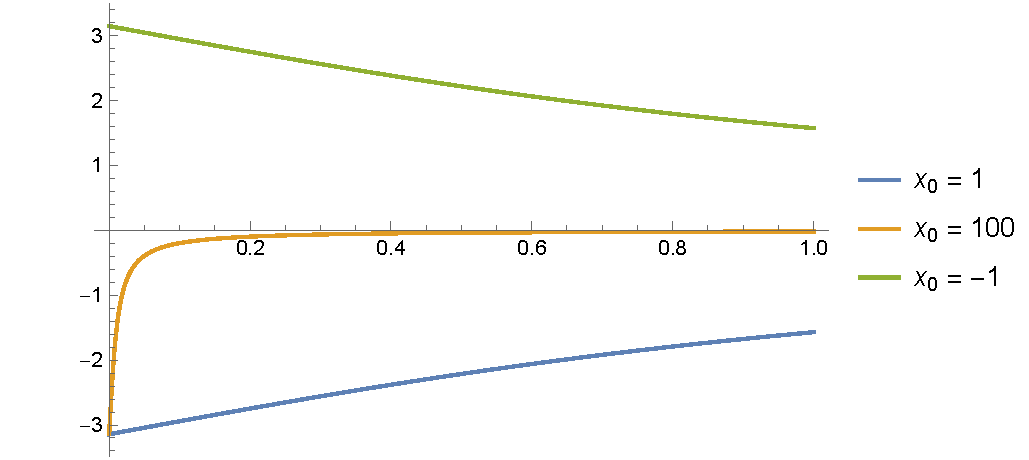
\includegraphics[width=0.8\linewidth]{free_phaseshift.pdf}
    \caption{The $Arg[r(k)]$ function.}
    \label{fig:free_phaseshift}
\end{figure}

\clearpage

\noindent
Remarkably, the physical content (\textit{i.e. \(R = 1\)}) of all the extensions is the same: the wall acts as a perfect reflector. However, the wave function that solves the problem is not independent of the self-adjoint extension, particularly the phase shift of the scattered state (\textit{i.e. $Arg[r(k)]$}), which is plotted in Fig.~\ref{fig:free_phaseshift}.

\vspace{4mm}
\noindent
Here we can introduce an experimental test that checks if the intuition from physics that leads us to impose the ${x_0} = 0$ self-adjoint extension is correct or not.
In fact, as long as an infinitely high wall is experimentally feasible, the dependence from the energy of the scattered wave function phase shift will act as a selector of some self-adjoint extensions. If the experiment says that the phase shift is independent from the energy of the wave function, our physical intuition of the boundary conditions is correct, if not we must take the specific self-adjoint extension that is suggested from the experiment.

\subsection{The Bound States}
With the usual boundary conditions from physics $\phi(0)=0$ (${x_0} = 0$), the presence of a bound state would have been excluded, hence no symmetry breaking. However, considering the generic self-adjoint extension, $\phi(0)$ is no longer restricted to zero, so we can suppose the existence of a bound state.

The wave function solution of the eigenvalue equation $-(\hbar^2/2m)d^2/dx^2 \phi = E \phi$ is:

\[
    \phi(x) = A e^{-\rho x}, \quad - \rho^2 := \frac{2mE}{\hbar^2},  \quad \rho > 0
\]

\noindent
For this wave function, Eq.~\eqref{half_BC} implies \((1 + {x_0}\rho)A = 0\). Since we want to find a non-zero solution: $A \neq 0$, this implies ${x_0}\rho = -1$.

Since $\rho$ should be positive, a bound state with \(\rho = -1/{x_0}\) is only possible when \({x_0} < 0\). So we've found that exist an infinite set of self-adjoint extensions that allows a single bound state, the formula for its energy is as we expected from Eq.~\eqref{eq:free_par_dimensional}.

\vspace{4mm}
\noindent
Now that we are delving into the mathematical aspects of the problem, it's important to note that considering the physical boundary conditions does not result in an anomaly. This is because the physics-motivated boundary conditions already render the Hamiltonian self-adjoint. This specific self-adjoint extension preserves scale invariance, and the theory does not admit bound states.

Conversely, different self-adjoint extensions do not preserve scale invariance. Therefore, in these cases, the presence of a bound state poses no problem.

\clearpage

\noindent
Its energy and normalized wave function are:

\[
    E = - \frac{\hbar^2}{2m{x_0}^2},  \quad {x_0} < 0,  \quad \phi(x) = \sqrt{\frac{2}{|{x_0}|}}e^{-x/|{x_0}|}
\]

\begin{figure}
    \centering
    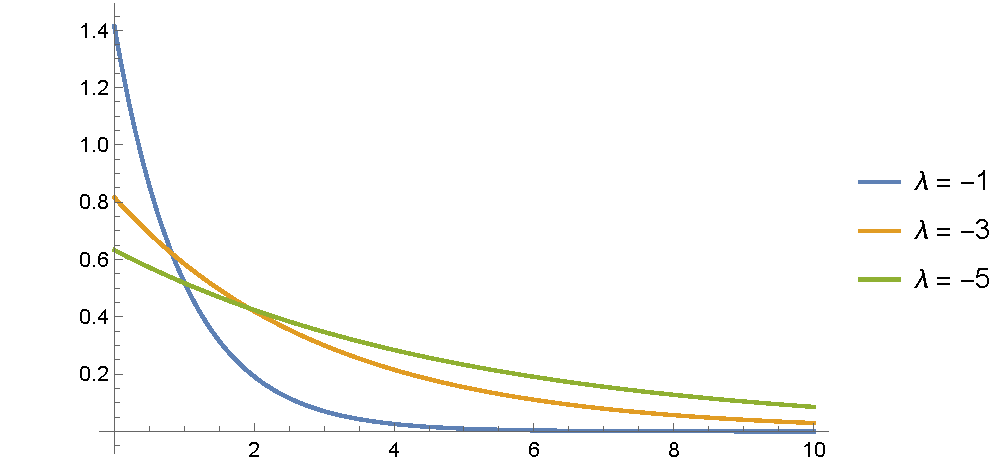
\includegraphics[width=0.8\linewidth]{free_boundstate.pdf}
    \caption{The $\phi(x)$ function.}
    \label{fig:free_boundstate}
\end{figure}

\noindent
Here again we can introduce an experimental test that checks if the intuition from physics that leads us to impose the ${x_0} = 0$ self-adjoint extension is correct or not.
In fact, as long as an infinitely high wall is experimentally feasible, the existence (or non-existence) of this negative energy will act as a selector of some self-adjoint extensions. If the experiment rules out the negative energy state, our intuition could be correct but there are still many possible extensions with \({x_0} \geq 0\). If not, our intuition would have been surely wrong since we've found a unique bound state (plotted in Fig.~\ref{fig:free_boundstate}).

\clearpage

\subsection*{Conclusion}
This chapter provided a simple example of the self-adjoint extension method. Therefore, from a physical perspective, we can employ this method to experimentally verify whether the boundary conditions we have traditionally used accurately describe the examined problem, considering that from a mathematical standpoint, the choice of a self-adjoint extension is arbitrary.

However, if we assume that our physical intuition is correct, the choice would be ${x_0} = 0$, thus preserving scale invariance and its associated consequences: an energy-independent phase shift and the absence of bound states.

\paragraph*{What if our intuition had resulted in an ill-defined problem?}
If, absurdly, our physical intuition had led us to define the boundary condition as $\psi(0) = 1$ (which renders our Hamiltonian operator non-self-adjoint), scale invariance would still be maintained. 
Consequently, based on scale invariance, we would have concluded that there is an energy-independent phase shift and no allowed bound states. 
Nevertheless, since the problem, as posed, doesn't have a self-adjoint Hamiltonian, it would have necessitated a self-adjoint extension.

Mathematically, this would have led us to the same conclusion we have reached in the discussion of this section—namely, a theory that, in general, is not scale-invariant. 
Hence, we would have broken scale invariance symmetry upon quantization, resulting in an anomalous symmetry breaking.

\vspace{4mm}
\noindent
The process we've outlined here is the analogous of what we will discuss in the next section.